\documentclass[output=paper]{langscibook}
\ChapterDOI{10.5281/zenodo.6393807}
\title{A phylogenetic classification of Luyia language varieties}

\author[Michael R. Marlo and others]
  {
    Michael R. Marlo\affiliation{University of Missouri} and 
    Rebecca Grollemund\affiliation{University of Missouri} and 
    Thanh Nguyen\affiliation{University of Missouri} and 
    Erik Platner\affiliation{University of Missouri} and 
    Sarah Pribe\affiliation{Ohio State University} and 
    Alexa Thein\affiliation{Washington University in St. Louis}
  }

\abstract{This paper presents the results of a comparative study of the Luyia cluster of Bantu languages spoken in western Kenya and eastern Uganda. We propose a new classification of Luyia and neighboring languages using phylogenetic methods. Our study is based on a 200-item wordlist of basic vocabulary, representing 33 language varieties from the Luyia cluster and its closest neighbors, including Ganda, Gwere, and Soga to the west, and Gusii and Kuria to the south. Our results are broadly consistent with past classifications by \citet{mould_comparative_1976,mould_greater_1981} and \citet{williams_lexico-statistical_1973}, but refine our understanding of the relatedness of the target languages by employing more extensive data from more languages within the Luyia cluster and others in the region.}
 
\begin{document}
\lehead{Michael R. Marlo et al.}
\maketitle
\section{Introduction} 
\label{sec:1:Introduction}

The Luyia language cluster consists of around 20 Bantu language varieties spoken in western Kenya and eastern Uganda. A map with several Luyia varieties and neighboring Bantu languages is shown in Figure \ref{fig:2:MapOfLuyia}. The languages that we refer to as part of the Luyia cluster are circled. This includes the Kenyan language varieties spoken by members of ``Luyia" or ``Luhya" ethnic communities that were politically united in the first half of the 20th century (see \cite{macarthur_cartography_2016}) as well as closely related linguistic varieties on the Ugandan side of the border that were not part of the ethnopolitical unification that took place in Kenya. A second map of Kenyan Luyia varieties from \citet[35]{heine_language_1980} is given in Figure \ref{fig:10:KenyanLuyia}.

\begin{figure}
  \caption{Map of the Luyia language cluster and its nearest neighboring Bantu languages\label{fig:2:MapOfLuyia}}
  \includegraphics[width=.66\textwidth]{figures/Luyia-clusters.pdf}
\end{figure}

\begin{figure}
  \caption{Map of Kenyan Luyia varieties \citep[35]{heine_language_1980}\label{fig:10:KenyanLuyia}}
  \includegraphics[width=.66\textwidth]{figures/Kenyan-Luyia-Varieties.pdf}
\end{figure}

The overarching goals of this project are to understand the relationship between the languages of the Luyia cluster and their closest neighbors and to understand the internal structure of the Luyia cluster. To achieve this goal, we propose a new classification of Luyia and its nearest neighbors using phylogenetic methods.  

\section{Prior classifications of Luyia}\label{sec:2:Prior_classifications}\largerpage

In this section, we provide a detailed overview of prior classifications of Luyia. These include geolinguistic classifications in \S\ref{sec:2.1:Geolinguistic_classifications}, genetic classifications in \S\ref{sec:2.2:Genetic_classifications}, a “dialectometrical” classification in \S\ref{sec:2.3:Dialectometrical_classification}, and the referential classification found in \emph{Glottolog} in \S\ref{sec:2.4:Referential_classification}. We conclude the section by identifying some lingering questions about specific varieties of Luyia mentioned in prior classifications in \S\ref{sec:2.5:Issues_in_prior_classifications}.

\subsection{Geolinguistic classifications \citep{guthrie_classification_1948,guthrie_comparative_1967,maho_nugl_2009,lewis_ethnologue:_2016}}
\label{sec:2.1:Geolinguistic_classifications}

The first geolinguistic classification of Luyia was established by  \citet{guthrie_classification_1948,guthrie_comparative_1967} and updated by linguists in Tervuren. These results, which were largely adopted by the \textit{Ethnologue} \citep{lewis_ethnologue:_2016}, are presented in an accessible way in \citet{maho_nugl_2009}. In these classifications, most language varieties of the Luyia cluster fall under JE30, the Masaaba-Luyia Group, shown in Table \ref{tab:1:JE30}. Within this classification, a large number of central Kenyan Luyia varieties fall within JE32, the so-called ``Lu(h)yia cluster".

\begin{table}
\caption{JE30: Masaaba-Luyia Group \citep{maho_nugl_2009}}
\label{tab:1:JE30}
 \begin{tabular}{lll} 
  \lsptoprule
  Bantu Code & Name & ISO Code \\ 
  \midrule
  JE31  &   Masaaba cluster &    [myx]\\
  JE31a  &   Gisu &   [myx]\\
  JE31b  &  Kisu  &  [myx]\\
  JE31c  & Bukusu  & [bxk] \\
  JE31D  & Syan  &  \\
  JE31E  & Tachoni  & [lts] \\
  JE31F  & Dadiri  & [myx] \\
  JE31G  & Buya  & [myx] \\
  JE32  & Lu(h)yia cluster  & [luy] \\
  JE32a  & Wanga  & [lwg] \\
  JE32b  & Tsotso  & [lto] \\
  JE32C  & Marama  & [lrm] \\
  JE32D  & Kisa  & [lks] \\
  JE32E  & Kabarasi  & [lkb] \\
  JE32F  & Nyala East & [nle] \\
  JE33  & Nyore  & [nyd] \\
  JE34  & Saamia  & [lsm] \\
  JE341  & Khayo  & [lko] \\
  JE342  & Marachi  & [lri] \\
  JE343  & Songa  &  \\
  JE345  & Nyole  & [nuj] \\
  \lspbottomrule
 \end{tabular}
\end{table}

Many broad aspects of this classification are uncontroversial -- for instance, the fact that the language varieties of JE30 should be grouped together. One aspect of the Guthrie/Maho classification that is controversial is the placement of a few language varieties that we consider part of the Luyia cluster outside of the JE30 decimal series. As shown in Table \ref{tab:2:JE40}, the southeastern varieties Isukha (JE412), Itakho (JE411), Logooli (JE41), and Tiriki (JE413) are in JE40, the Logooli-Kuria Group, along with Gusii (JE42) and Kuria (JE43), and several other languages of the Mara region of northwest Tanzania. Additionally, as shown in Table \ref{tab:3:JE10}, \citet{maho_nugl_2009} places Nyala West in JE18, part of JE10 along with Soga and Ganda.

\begin{table}
\caption{JE40: Logooli-Kuria Group \citep{maho_nugl_2009}}
\label{tab:2:JE40}
 \begin{tabular}{lll} 
  \lsptoprule
  Bantu Code & Name & ISO Code \\ 
  \midrule
  JE401  & Ngoreme  & [ngq] \\
  JE402  & Ikizu  & [ikz] \\
  JE403  & Suba  & [suh] \\
  JE404  & Shashi  & [szk] \\
  JE405  & Kabwa  & [cwa] \\
  JE406  & Singa†  & [sgm] \\
  JE407  & Ware†  & [wre] \\
  JE41  & Logooli  & [rag] \\
  JE411  & Itakho  & [ida] \\
  JE412  & Isukha  & [ida] \\
  JE413  & Tiriki  & [ida] \\
  JE42  & Gusii  & [guz] \\
  JE43  & Kuria  & [kuj] \\
  JE431  & Simbiti  & [ssc] \\
  JE432  & Hacha  & [ssc] \\
  JE433  & Surwa  & [ssc] \\
  JE434  & Sweta  & [ssc] \\
  JE44  & Zanaki  & [zak] \\
  JE45  & Ikoma-Nata-Isenye  & [ntk] \\
  \lspbottomrule
 \end{tabular}
\end{table}

Nyala West is sometimes referred to as ``West Nyala" and Nyala East is sometimes referred to as ``East Nyala" or ``Nyala K", referring to Kakamega -- the name of the county where Nyala East is spoken. As shown in Figure \ref{fig:10:KenyanLuyia}, Nyala East is surrounded by several other Luyia varieties: Bukusu, Tachoni, Kabarasi, Wanga, and Tsootso. Nyala West is spoken in Busia County adjacent to the southwestern variety Saamia. 

In 2007, Luyia was introduced as a “macrolanguage” in the \textit{Ethnologue}, and many of the Luyia varieties were recognized with distinct ISO codes. As part of this change, Nyala East was renamed ``Olunyala" (i.e.\ ``Nyala" without the cl.\ 11 noun class prefix), and although Nyala West was not mentioned in \mbox{ISO\,639-3} Change Request Number 2007-171, Nyala West was also included as part of Nyala in the changes implemented in the ISO\,639-3 reclassification. Nyala West and Nyala East were thus unified as part of JE32 in the 16th edition of \textit{Ethnologue}, but this seems to have been an accident resulting from the shared language name and the lack of mention of Nyala West in the change request. A subsequent ISO change request (2014-001) to reintroduce Nyala East and Nyala West as separate language varieties with distinct ISO codes was rejected, citing a lack of linguistic evidence. (The authors of the change request failed to cite \citet{heine_language_1980}, which includes Nyala East in the northern-central Bukusu-Wanga cluster and Nyala West in the southwestern Saamia-Nyala cluster.) This decision failed to recognize that the merger of these two languages 7 years earlier had also been done without any linguistic evidence or even a specific request to merge the two language varieties under one name.

\begin{table}
\caption{JE10: Nyoro-Ganda Group \citep{maho_nugl_2009}}
\label{tab:3:JE10}
 \begin{tabular}{lll} 
  \lsptoprule
  Bantu Code & Name & ISO Code \\ 
  \midrule
  JE101  & Gungu  & [rub] \\
  JE102  & Talinga-Bwisi  & [tlj] \\
  JE103  & Ruli  & [ruc] \\
  JE11  & Nyoro  & [nyo] \\
  JE12  & Tooro  & [ttj] \\
  JE121  & Hema  & [nlx] \\
  JE13  & Nkore  & [nyn] \\
  JE14  & Kiga  & [cgg] \\
  JE15  & Ganda  & [lug] \\
  JE16  & Soga  & [xog] \\
  JE16  & Kenyi  & [lke] \\
  JE17  & Gwere  & [gwr] \\
  JE18  & Nyala West  & [nle] \\
  \lspbottomrule
 \end{tabular}
\end{table}

\subsection{Genetic classifications \citep{mould_comparative_1976,mould_greater_1981,williams_lexico-statistical_1973,nurse_bantu_1980}}
\label{sec:2.2:Genetic_classifications}

The first genetic classification of Luyia language varieties was done by \citet{williams_lexico-statistical_1973}, who presents a relatively extensive internal classification of Luyia with data from 16 Luyia varieties. \citet{williams_lexico-statistical_1973} primarily uses lexicostatistic methods and the 200-item Swadesh list.\footnote{\citet{williams_lexico-statistical_1973} also identifies some phonological correspondences across varieties and compares the noun class prefixes across Luyia varieties.} Lexicostatistics -- the method developed by \citet{swadesh-1952-lexicostatistic-dating} -- measures the percentages of shared cognates by comparing the similarity of words from the basic vocabulary of Swadesh between two or more related languages. Williams' (\citeyear{williams_lexico-statistical_1973}) approach yields a geographically-based clustering of varieties, shown in Figure \ref{fig:7:Williams1973}, which has a flat structure with five branches: Western, Northern, Central, Eastern, and Southeastern. Note that in contrast with the Guthrie/Maho system, the southeastern varieties Isukha, Itakho, Logooli, and Tiriki, and the southwestern variety Nyala West are treated as part of Luyia in William's (\citeyear{williams_lexico-statistical_1973}) classification.

\vfill
\begin{figure}[H]
  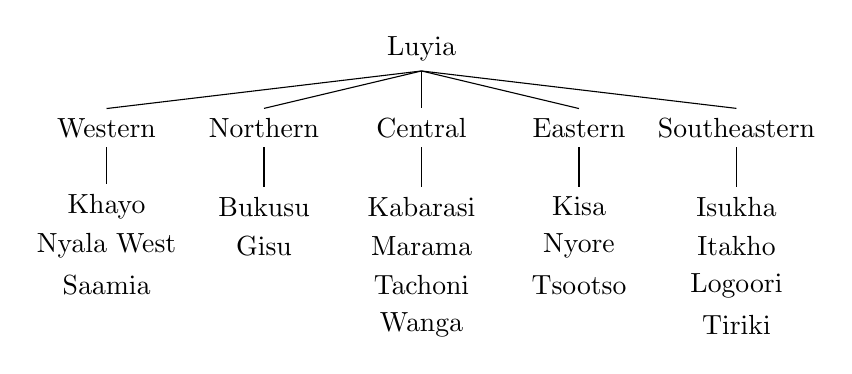
\begin{tikzpicture}
   
   \node (Western) at (-4,2.5) [] {Western};
   \node (Khayo) at (-4,1.5) [] {Khayo};
   \node (NyalaW) at (-4,1.0) [] {Nyala West};
   \node (Saamia) at (-4,0.5) [] {Saamia};

   \node (Northern) at (-2,2.5) [] {Northern};
   \node (Bukusu) at (-2,1.5) [] {Bukusu};
   \node (Gisu) at (-2,1.0) [] {Gisu};

   \node (Luyia) at (0,3.5) [] {Luyia};
   \node (Central) at (0,2.5) [] {Central};
   \node (Kabarasi) at (0,1.5) [] {Kabarasi};
   \node (Marama) at (0,1.0) [] {Marama};
   \node (Tachoni) at (0,0.5) [] {Tachoni};
   \node (Wanga) at (0,0.0) [] {Wanga};

   \node (Eastern) at (2,2.5) [] {Eastern};
   \node (Kisa) at (2,1.5) [] {Kisa};
   \node (Nyore) at (2,1.0) [] {Nyore};
   \node (Tsootso) at (2,0.5) [] {Tsootso};
   
   \node (Southeastern) at (4,2.5) [] {Southeastern};
   \node (Isukha) at (4,1.5) [] {Isukha};
   \node (Itakho) at (4,1.0) [] {Itakho};
   \node (Logoori) at (4,0.5) [] {Logoori};
   \node (Tiriki) at (4,0.0) [] {Tiriki};

   \draw [] (Luyia.south) -- (Western.north);
   \draw [] (Luyia.south) -- (Northern.north);
   \draw [] (Luyia.south) -- (Central.north);
   \draw [] (Luyia.south) -- (Eastern.north);
   \draw [] (Luyia.south) -- (Southeastern.north);
   
   \draw [] (Western.south) -- (Khayo.north);
   \draw [] (Northern.south) -- (Bukusu.north);
   \draw [] (Central.south) -- (Kabarasi.north);
   \draw [] (Eastern.south) -- (Kisa.north);
   \draw [] (Southeastern.south) -- (Isukha.north);
  
   \end{tikzpicture}
   
  \caption{Williams' (\citeyear{williams_lexico-statistical_1973}) classification of Luyia}
  \label{fig:7:Williams1973}
\end{figure}
\vfill\pagebreak

\begin{sloppypar}
Mould’s (\citeyear{mould_comparative_1976,mould_greater_1981}) classifications generally accord with \citet{williams_lexico-statistical_1973}, though Mould worked with different languages. Using a 200-item wordlist, \citet{mould_comparative_1976,mould_greater_1981} carried out a lexicostatistic analysis including five Luyia varieties (Bukusu, Itakho, Logooli, Saamia, and Wanga) along with Ganda and Soga to the west and Gusii to the south. Mould’s (\citeyear{mould_comparative_1976,mould_greater_1981}) results, summarized in Figure \ref{fig:3:Mould1981-lexicostatistics}, show the overall unity of Luyia, as the varieties we consider part of the Luyia cluster are more similar to one another than they are to Ganda, Soga, and Gusii. Internally within Luyia, the Southeastern varieties Itakho and Logoori branch off from Saamia, Wanga, and Bukusu, which is divided into a Northern branch with Bukusu and a Western-Central branch with Saamia and Wanga.   
\end{sloppypar}

\begin{figure}
  \centering
  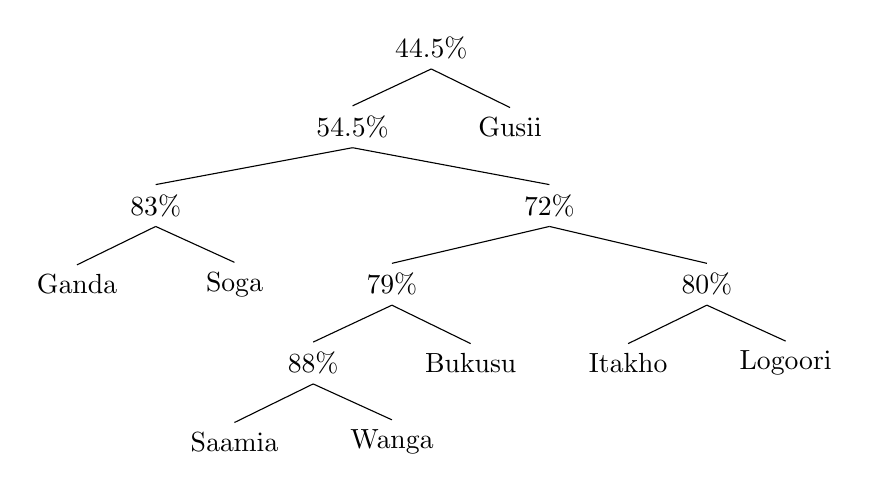
\begin{tikzpicture}

   \node (44) at (-0.5,5.0) [] {44.5\%} ;
   \node (Gusii) at (0.5,4.0) [] {Gusii} ;
   \node (54) at (-1.5,4.0) [] {54.5\%} ;
   \node (72) at (1,3.0) [] {72\%};
   \node (83) at (-4,3.0) [] {83\%};
   \node (Ganda) at (-5,2.0) [] {Ganda};
   \node (Soga) at (-3,2.0) [] {Soga};
   \node (79) at (-1,2.0) [] {79\%};
   \node (80) at (3,2.0) [] {80\%};
   \node (Itakho) at (2,1.0) [] {Itakho};
   \node (Logoori) at (4,1.0) [] {Logoori};
   \node (Bukusu) at (0,1.0) [] {Bukusu};
   \node (88) at (-2,1.0) [] {88\%};
   \node (Saamia) at (-3,0) [] {Saamia};
   \node (Wanga) at (-1,0) [] {Wanga};

   \draw [] (44.south) -- (54.north);
   \draw [] (44.south) -- (Gusii.north);
 
   \draw [] (54.south) -- (83.north);
   \draw [] (54.south) -- (72.north);

   \draw [] (83.south) -- (Ganda.north);
   \draw [] (83.south) -- (Soga.north);

   \draw [] (72.south) -- (79.north);
   \draw [] (72.south) -- (80.north);

   \draw [] (79.south) -- (88.north);
   \draw [] (79.south) -- (Bukusu.north);

   \draw [] (80.south) -- (Itakho.north);
   \draw [] (80.south) -- (Logoori.north);

   \draw [] (88.south) -- (Saamia.north);
   \draw [] (88.south) -- (Wanga.north);

   \end{tikzpicture}
   
  \caption{Mould’s (\citeyear[185]{mould_greater_1981}) classification of Luyia based on lexicostatistics}
  \label{fig:3:Mould1981-lexicostatistics}
\end{figure}

\citet[201]{mould_greater_1981} also considers sound change in creating a second tree with similar results, shown in Figure \ref{fig:4:Mould1981-sound-change}. There are two differences in this tree: (i) Logoori branches off from Itakho at a higher level in the tree, and (ii) Bukusu, Saamia, and Wanga are not subdivided further. \citet[201]{mould_greater_1981} also computes a third tree based on a comparison of tense/aspect markers; its results are identical to the tree based on sound change.

\begin{figure}
  \centering
  \begin{tikzpicture}

   \node (North-Nyanza-Greater-Luyia) at (0.0,5.0) [] {North Nyanza-Greater Luyia};
   \node (*p>ɸ>w) at (0.0,4.5) [] {*p > ɸ > w̥};

   \node (North-Nyanza) at (-3,3.5) [] {North Nyanza};
   \node (*p>w) at (-3,3.0) [] {*p > w};
   \node (independent) at (-3,2.5) [] {(developed independently)};
   \node (Ganda) at (-4,1.5) [] {Ganda};
   \node (Soga) at (-2,1.5) [] {Soga};
   
   \node (Greater-Luyia) at (3.0,3.5) [] {Greater Luyia};
   \node (*NC) at (3.0,3.0) [] {*NC̥ >NC};
   \node (*N>∅) at (3.0,2.5) [] {*N > ∅ before fricatives};

   \node (Logoori) at (4.5,1.5) [] {Logoori};
   
   \node (Luyia) at (1.5,1.5) [] {Luyia};
   \node (Luyia-Law) at (1.5,1.0) [] {Luyia Law};

   \node (Bukusu-Saamia-Wanga) at (-1.0,0.0) [] {Bukusu-Saamia-Wanga};
   \node (*v>f) at (-1.0,-0.5) [] {*v>f, *z>s};
   
   \node (Itakho) at (3.0,0.0) [] {Itakho};

   \node (Bukusu) at (-3.0,-1.5) [] {Bukusu};
   \node (Saamia) at (-1.0,-1.5) [] {Saamia};
   \node (Wanga) at (1.0,-1.5) [] {Wanga};

   \draw [] (*p>ɸ>w.south) -- (Greater-Luyia.north);
   \draw [] (*p>ɸ>w.south) -- (North-Nyanza.north);
 
   \draw [] (*N>∅.south) -- (Luyia.north);
   \draw [] (*N>∅.south) -- (Logoori.north);

   \draw [] (independent.south) -- (Ganda.north);
   \draw [] (independent.south) -- (Soga.north);

   \draw [] (Luyia-Law.south) -- (Bukusu-Saamia-Wanga);
   \draw [] (Luyia-Law.south) -- (Itakho.north);

   \draw [] (*v>f.south) -- (Bukusu.north);
   \draw [] (*v>f.south) -- (Saamia.north);
   \draw [] (*v>f.south) -- (Wanga.north);

   \end{tikzpicture}
   
  \caption{Mould’s (\citeyear[201]{mould_greater_1981}) classification of Luyia based on sound change}
  \label{fig:4:Mould1981-sound-change}
\end{figure}

Nurse \& Philippson's (\citeyear{nurse_bantu_1980}) classification is based on a lexicostatistical study with a 400-item wordlist. It includes four Luyia language varieties and essentially gives the same results as \citet{mould_comparative_1976,mould_greater_1981} but with fewer languages. As shown in Figure \ref{fig:6:NursePhilippson1980}, there is a geographical split that divides Saamia and Bukusu from Itakho and Logoori. \citet{nurse_bantu_1980} treat this as a North-South split, though ``West" vs. ``East" appears to us to be equally tenable labels for the two groups.

\begin{figure}
  \centering
  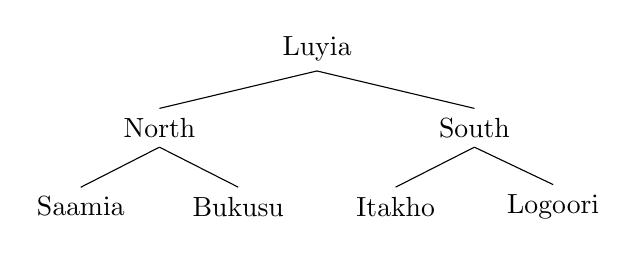
\begin{tikzpicture}
 
   \node (Luyia) at (0,2.0) [] {Luyia};
   
   \node (North) at (-2,1.0) [] {North};
   \node (Saamia) at (-3,0) [] {Saamia};
   \node (Bukusu) at (-1,0) [] {Bukusu};

   \node (South) at (2,1.0) [] {South};
   \node (Itakho) at (1,0) [] {Itakho};
   \node (Logoori) at (3,0) [] {Logoori};
   
   \draw [] (Luyia.south) -- (North.north);
   \draw [] (Luyia.south) -- (South.north);
   
   \draw [] (North.south) -- (Saamia.north);
   \draw [] (North.south) -- (Bukusu.north);

   \draw [] (South.south) -- (Itakho.north);
   \draw [] (South.south) -- (Logoori.north);

   \end{tikzpicture}
   
  \caption{\citeauthor{nurse_bantu_1980}’s (1980) classification of Luyia}
  \label{fig:6:NursePhilippson1980}
\end{figure}

% Other classifications have not specifically compared Luyia with non-Luyia but have shed light on the internal structure of Luyia, focusing primarily on Kenyan varieties of Luyia.

\subsection{Dialectometrical classification \citep{heine_language_1980}}
\label{sec:2.3:Dialectometrical_classification}

The classification of 15 varieties of Kenyan Luyia by \citet{heine_language_1980} is part of a large-scale study of languages in Kenya, which includes a wordlist of 640 concepts, documentation of each variety's phonological system, and basic features of grammar \citep[9]{heine_language_1980}. Their classification of Luyia is an areal grouping, based on ``geographical and synchronic dialectal proximity \citep[13]{heine_language_1980}.'' \citet[32]{heine_language_1980} state that the Luyia varieties, ``neither form a single dialect cluster nor even represent dialects of variations of a single language. The term [Luyia] as such is geographical and has no further dialectological significance.” Internal subgroupings are based on ``dialectal proximity", which measures the degree of of linguistic similarity in linguistic features, e.g.\ isoglosses, across dialect clusters.

The four subgroupings established by \citet{heine_language_1980} are shown in Figure \ref{fig:8:Heine-Mohlig1980}. Logooli is viewed as a ``separate language", and three other ``cluster[s] of dialects" are identified: a Southwestern cluster, a Central-Northern cluster, and a Southeastern cluster. The separation of Logoori from the Southeastern languages and the inclusion of Central and Northern varieties in a single larger branch is similar to Mould's (\citeyear{mould_comparative_1976,mould_greater_1981}) classifications but different from \citet{williams_lexico-statistical_1973}.

\begin{figure}
  \centering
  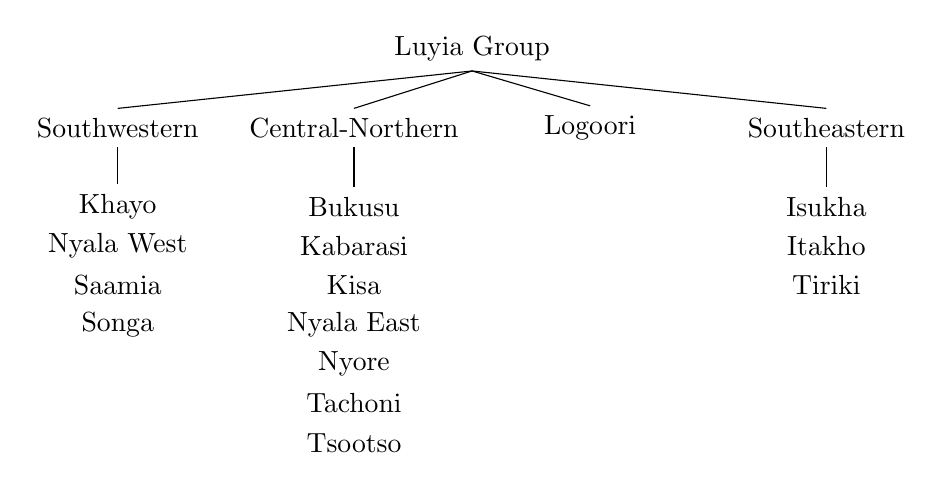
\begin{tikzpicture}
   
   \node (Southwestern) at (-4.5,4.0) [] {Southwestern};
   \node (Khayo) at (-4.5,3.0) [] {Khayo};
   \node (NyalaW) at (-4.5,2.5) [] {Nyala West};
   \node (Saamia) at (-4.5,2.0) [] {Saamia};
   \node (Songa) at (-4.5,1.5) [] {Songa};

   \node (Central) at (-1.5,4.0) [] {Central-Northern};
   \node (Bukusu) at (-1.5,3.0) [] {Bukusu};
   \node (Kabarasi) at (-1.5,2.5) [] {Kabarasi};
   \node (Kisa) at (-1.5,2.0) [] {Kisa};
   \node (NyalaE) at (-1.5,1.5) [] {Nyala East};
   \node (Nyore) at (-1.5,1.0) [] {Nyore};
   \node (Tachoni) at (-1.5,0.5) [] {Tachoni};
   \node (Tsootso) at (-1.5,0.0) [] {Tsootso};
   
   \node (Luyia) at (0,5.0) [] {Luyia Group};

   \node (Logoori) at (1.5,4.0) [] {Logoori};

   \node (Southeastern) at (4.5,4.0) [] {Southeastern};
   \node (Isukha) at (4.5,3.0) [] {Isukha};
   \node (Itakho) at (4.5,2.5) [] {Itakho};
   \node (Tiriki) at (4.5,2.0) [] {Tiriki};

   \draw [] (Luyia.south) -- (Southwestern.north);
   \draw [] (Luyia.south) -- (Central.north);
   \draw [] (Luyia.south) -- (Logoori.north);
   \draw [] (Luyia.south) -- (Southeastern.north);

   \draw [] (Southwestern.south) -- (Khayo.north);
   \draw [] (Central.south) -- (Bukusu.north);
   \draw [] (Southeastern.south) -- (Isukha.north);
  
   \end{tikzpicture}
   
  \caption{\citeauthor{heine_language_1980}’s (1980) classification of Luyia}
  \label{fig:8:Heine-Mohlig1980}
\end{figure}

The authors indicate that the linguistic data undergirding the atlas would be published in future volumes, but no subsequent studies on Luyia languages were published from the project. See \citet{heine_language_2013} for a later overview of the \textit{Language and Dialect Atlas of Kenya} project and see Möhlig's  (\citeyear{mohlig-1985-review-of-angogo-kanyoro-1983}) review of \citet{angogokanyoro1983} for some additional comments on his “dialectometrical” analysis of the Luyia area, which includes the identification of three ``dialect continua": Marachi-Khayo in the west, Kabarasi-Tachoni-Nyala East in the east, and Nyore in the south. 

% The \textit{Language and Dialect Atlas of Kenya} monograph series generated numerous volumes e.g.\ \citep{heine1982language} on Bantu languages spoken around Mt.\ Kenya. 

\subsection{Referential classification \citep{glottolog}}
\label{sec:2.4:Referential_classification}

A recent referential classification of ``Greater Luyia", which includes both Kenyan and Ugandan language varieties, is found in the \textit{Glottolog} \citep{glottolog}. The \textit{Glottolog} 4.3 classification, which is based on secondary materials -- primarily \citet{mould_greater_1981} -- is shown in Figure \ref{fig:9:Glottolog}. As noted above, \citet{mould_greater_1981} deals with only a small subset of the language varieties represented in the \textit{Glottolog} classification. It appears that the many other language varieties present in the \textit{Glottolog} classification are populated from uncited sources, with the \textit{Ethnologue} database being a possible source. The \textit{Glottolog} represents the prior classification with the most Luyia language varieties displayed in a tree format, but it is not a genetic classification based on original data, and the justification for many aspects of its structure is unclear. 

Our representation of the \textit{Glottolog} classification given here in Figure \ref{fig:9:Glottolog} differs from the original in a few ways. First, we harmonized some language names (e.g. ``Idakho" → ``Itakho", ``Kabras" → ``Kabarasi"), and we eliminated the cl.\ 11 \textit{ulu-} noun class prefix from the languages under the Masaaba node. 

\begin{figure}
  \centering
  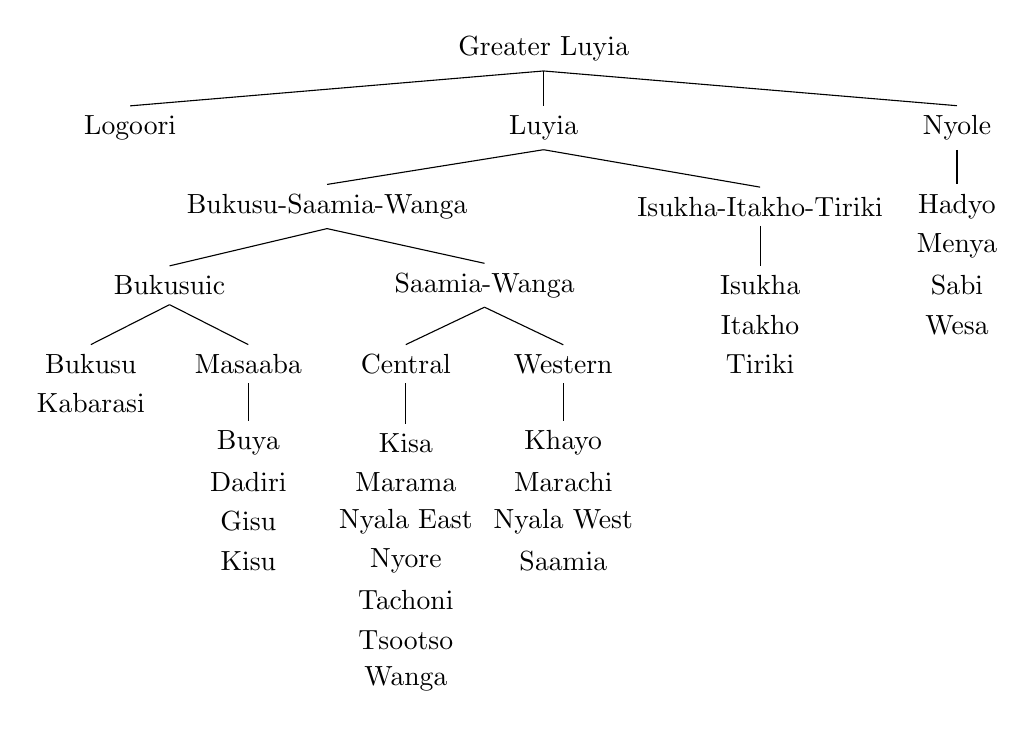
\begin{tikzpicture}
   
   \node (GreaterLuyia) at (0,3.5) [] {Greater Luyia};
   
   \node (Logoori) at (-5.25,2.5) [] {Logoori};
   
   \node (Luyia) at (0,2.5) [] {Luyia};
   
   \node (Bukusu-Saamia-Wanga) at (-2.75,1.5) [] {Bukusu-Saamia-Wanga};
   
   \node (Bukusuic) at (-4.75,0.5) [] {Bukusuic};
   \node (Bukusu) at (-5.75,-0.5) [] {Bukusu};
   \node (Kabarasi) at (-5.75,-1.0) [] {Kabarasi};
   \node (Masaaba) at (-3.75,-0.5) [] {Masaaba};
   \node (Buya) at (-3.75,-1.5) [] {Buya};
   \node (Dadiri) at (-3.75,-2.0) [] {Dadiri};
   \node (Gisu) at (-3.75,-2.5) [] {Gisu};
   \node (Kisu) at (-3.75,-3.0) [] {Kisu};
   
   \node (Saamia-Wanga) at (-0.75,0.5) [] {Saamia-Wanga};
   \node (Central) at (-1.75,-0.5) [] {Central};
   \node (Kisa) at (-1.75,-1.5) [] {Kisa};
   \node (Marama) at (-1.75,-2.0) [] {Marama};
   \node (NyalaEast) at (-1.75,-2.5) [] {Nyala East};
   \node (Nyore) at (-1.75,-3.0) [] {Nyore};
   \node (Tachoni) at (-1.75,-3.5) [] {Tachoni};
   \node (Tsootso) at (-1.75,-4.0) [] {Tsootso};
   \node (Wanga) at (-1.75,-4.5) [] {Wanga};
   \node (Western) at (0.25,-0.5) [] {Western};
   \node (Khayo) at (0.25,-1.5) [] {Khayo};
   \node (Marachi) at (0.25,-2.0) [] {Marachi};
   \node (NyalaWest) at (0.25,-2.5) [] {Nyala West};
   \node (Saamia) at (0.25,-3.0) [] {Saamia}; 

   \node (Isukha-Itakho-Tiriki) at (2.75,1.5) [] {Isukha-Itakho-Tiriki};
   \node (Isukha) at (2.75,0.5) [] {Isukha};
   \node (Itakho) at (2.75,0.0) [] {Itakho};
   \node (Tiriki) at (2.75,-0.5) [] {Tiriki};
   
   \node (Nyole) at (5.25,2.5) [] {Nyole};
   \node (Hadyo) at (5.25,1.5) [] {Hadyo};
   \node (Menya) at (5.25,1.0) [] {Menya};
   \node (Sabi) at (5.25,0.5) [] {Sabi};
   \node (Wesa) at (5.25,0.0) [] {Wesa};

   \draw [] (GreaterLuyia.south) -- (Logoori.north);
   \draw [] (GreaterLuyia.south) -- (Luyia.north);
   \draw [] (GreaterLuyia.south) -- (Nyole.north);

   \draw [] (Luyia.south) -- (Isukha-Itakho-Tiriki.north);
   \draw [] (Luyia.south) -- (Bukusu-Saamia-Wanga.north);

   \draw [] (Bukusu-Saamia-Wanga.south) -- (Bukusuic.north);
   \draw [] (Bukusu-Saamia-Wanga.south) -- (Saamia-Wanga.north);   

   \draw [] (Bukusuic.south) -- (Bukusu.north);
   \draw [] (Bukusuic.south) -- (Masaaba.north);
   
   \draw [] (Masaaba.south) -- (Buya.north);
   
   \draw [] (Isukha-Itakho-Tiriki.south) -- (Isukha.north);
   \draw [] (Nyole.south) -- (Hadyo.north);

   \draw [] (Saamia-Wanga.south) -- (Central.north);
   \draw [] (Saamia-Wanga.south) -- (Western.north);
   
   \draw [] (Central.south) -- (Kisa.north);
   \draw [] (Western.south) -- (Khayo.north);
   
   \end{tikzpicture}
   
  \caption{Glottolog 4.3 classification of Luyia \citep{glottolog}}
  \label{fig:9:Glottolog}
\end{figure}

Second, two languages are listed in multiple locations in the \textit{Glottolog} tree, and we have retained the languages in only one position. Tachoni is given under a node for Bukusu where it is contrasted with ``Nuclear Bukusu" and under the Central Luyia node. We have not seen evidence for two distinct varieties of Tachoni. Following \citet[305]{odden_tachoni_2009}, who states that ``Tachoni most resembles “mainstream” Luhya varieties such as Tsootso, Nyala, Wanga, Kisa, and Marachi, least resembling Bukusu, [Gisu], and Logoori," we have included Tachoni only under the Central Luyia node, and we have simplified the Bukusu node, eliminating ``Nuclear Bukusu". Bukusu is also listed in two locations in the \textit{Glottolog} tree: under the ``Bukusuic" node with Kabarasi and under Masaaba, where presumably it refers to Ugandan Bukusu. Lacking evidence for a distinct form of Ugandan Bukusu, we have not included Bukusu under Masaaba.  

Third, Nyole and its subvarieties are considered ``Unclassified Luyia" in the \textit{Glottolog} and are listed as a highest level branch of Greater Luyia. We have maintained the position of Nyole within the tree but have removed the ``Unclassified Luyia" label, acknowledging here that further study of Nyole and other Bantu language varieties of eastern Uganda might place those languages in a different position within the tree. \citet{maho_nugl_2009} includes Nyole (JE345) within JE34, which makes it most similar to other southwestern varieties Saamia (JE34), Khayo (JE341), and Marachi (JE342); no other classifications indicate the position of Nyole within Greater Luyia, as far as we know.

Given that \citet{mould_greater_1981} is cited as the basis for the \textit{Glottolog} classification, it is not surprising that the \textit{Glottolog} tree reflects the results of \citet{mould_greater_1981} (see Figures \ref{fig:3:Mould1981-lexicostatistics}--\ref{fig:4:Mould1981-sound-change} above). However, as \citet{mould_greater_1981} includes only 5 language varieties of Greater Luyia (Logoori, Itakho, Bukusu, Wanga, Saamia), many details concerning the internal structure of Luyia are underspecified in \citet{mould_greater_1981}. These uncertain details include the grouping of other languages with those studied by Mould as well as decisions to subdivide \citegen{mould_greater_1981} groupings further.

Although it is unclear how the \textit{Glottolog} arrived at its classification, several aspects of its structure are consistent with the results of other research:

\begin{itemize}
    \item Setting off Logoori at the highest level of the tree follows Mould's (\citeyear[]{mould_greater_1981}) trees based on sound changes tense-aspect markers. This is also consistent with Heine \& Möhlig's (\citeyear{heine_language_1980}) treatment of Logoori as a separate language.
    
    \item The inclusion of Isukha and Tiriki alongside Itakho in a high-level southeastern branch of Luyia is consistent with the results of \citet{williams_lexico-statistical_1973} and \citet{heine_language_1980}.
    
    \item The inclusion of Masaaba varieties alongside Bukusu in a northern branch of Luyia is supported by \citet{williams_lexico-statistical_1973}.
    
    \item The division of Saamia-Wanga into a Central branch and Southwestern branch is supported by \citet{williams_lexico-statistical_1973}.
    
    \item The inclusion of Marama, Tachoni, and Wanga in the Central branch is consistent with the results of \citet{williams_lexico-statistical_1973}.
    
    \item The inclusion of Khayo, Nyala West, and Saamia follows both \citet{williams_lexico-statistical_1973} and \citet{heine_language_1980}.
\end{itemize}

A few aspects of the \textit{Glottolog} classification differ from other prior classifications:

\begin{itemize}
    \item The \textit{Glottolog} classification of Kabarasi with Bukusu in a Northern branch differs from the results of \citet{williams_lexico-statistical_1973}, which classifies Kabarasi with the Central varieties.
    
    \item \citet{williams_lexico-statistical_1973} subdivides the languages of the \textit{Glottolog} Central group into Central and Eastern subgroups.
    
    \item \citet{heine_language_1980} differs from \citet{mould_comparative_1976,mould_greater_1981}, \citet{williams_lexico-statistical_1973}, and \textit{Glottolog} in collapsing the Central and Northern groups.
    
    \item  No prior studies include Marachi, so it is unclear on what basis Marachi is included with the Western varieties in \textit{Glottolog}.
    
\end{itemize}

%  \citet{mould_greater_1981} does not include Isukha or Tiriki in his study.

% Mould's \citeyear[]{mould_greater_1981} tree based on lexicostastic information motivates a northern branch with Bukusu and a central-western Saamia-Wanga branch. It is unknown on what basis Masaaba is included with Bukusu in the \textit{Glottolog}. \citet{williams_lexico-statistical_1973} has an Eastern branch with Kisa, Nyore, and Tsootso, but these varieties are not set apart in the \textit{Glottolog}. It is also unknown what the \textit{Glottolog}'s basis is for subdividing the Saamia-Wanga branch into Central and Western branches because \citet{mould_greater_1981} does not include data on any of the other languages listed within these branches. 

\subsection{Issues in prior classifications}
\label{sec:2.5:Issues_in_prior_classifications}

There are a few questions about some of the specific varieties listed in past classifications. Within the Masaaba cluster, the \textit{Ethnologue} treats Gisu and Masaaba as alternative names for the same language, of which Kisu (JE31b) is another alternative name. We are doubtful that there are distinct language forms ``Gisu" vs.\ ``Kisu", but we have retained Maho's labels in Table \ref{tab:1:JE30} because distinct codes are given to the two language names. The \textit{Glottolog} also includes both ``Gisu" and ``Kisu", but we are not aware of any discussion of this distinction in the literature.

Buya (JE31G) and Dadiri (JE31F) are treated as dialects of Masaaba in \citet{maho_nugl_2009} and the \textit{Glottolog}. Despite the existence of an early grammar \citep{purvis_manual_1907}, a robust wordlist \citep{siertsema_masaba_1981}, and a book on Gisu\slash Masaaba dialect variation \citep{brown_phonological_1972}, there is little available information concerning the classification of Gisu\slash Masaaba language varieties. Similarly, we are unaware of materials dealing with the classification of the Nyole language varieties identified in the \textit{Glottolog}.

A further question concerns Syan, a variety described in \citet{huntingford_orusyan_1965} based on materials collected in 1924 from Syan migrant workers in Uasin Gishu province in Kenya. Huntingford confirmed that Syan people lived in Bulegenyi District in eastern Uganda as late as 1930, though other investigators reported not encountering a Syan ethnic group in that area. Syan is no longer listed in the most recent versions of the \textit{Ethnologue}, and we are not aware of any additional research on the language. Citing \citet{schoenbrun_great_1994}, the \textit{Glottolog} states that ``Syan is a missing language of the North Nyanza subgroup of Bantu, which [is] lexicostatistically too divergent" to be [mutually] intelligible [with] any other language in JE10 or JE20. In the \textit{Glottolog} classification, North Nyanza includes Ganda, Gwere, Kenyi, Lamogi, and Soga. \citet{maho_nugl_2009} however does classify Syan as part of JE31 (JE31D).

It is also unknown how Songa (JE343) fits in. The \textit{Ethnologue} lists it as a dialect of Saamia, and \citet[32]{heine_language_1980} include it as part of their Saamia-Nyala dialect cluster, with which it is geographically adjacent (see the map in Figure \ref{fig:10:KenyanLuyia}). \citet[32]{heine_language_1980}, who focus on languages in Kenya, list a population of 10,000 Songa speakers. This figure is consistent with the fact that the 1979 Kenyan census, cited by \citet[26]{were_siaya_1987}, identified 9,000 inhabitants of Usonga location in Siaya District. As reported in \citet[2-3]{marlo_verbal_2007}, Marlo attempted in 2006 to collect information on Songa, but it was unclear how the variety differed from Nyala West. Confusingly and possibly erroneously, various editions of the \textit{Ethnologue} (e.g.\ 13th edn.) identify 10,000 speakers of Songa in Uganda, but we have been unable to find any other sources that identify a Songa language variety of Uganda. As noted by \citet{marlo_luyia_2009}, a 2004 report by the SIL Language Assessment team on Gwe and Saamia in Busia District, Uganda \citep{anderson_lusamia-lugwe_2004}, does not mention Songa in its results. We have not seen any Songa data in the literature.

There is also at least one Luyia variety not listed in prior classifications, Tura, which is described in \citet{marlo_tura_2008}. Although the exact classification of this variety is unclear, it is geographically and linguistically most proximal to Bukusu, Khayo, and Wanga, and should fit in with the JE30 languages. 

A few communities of Greater Luyia have offshoots in the diaspora. \citet{marlo_sketch_2017} provide a description of a variety of Nyole spoken in southern Busoga, Uganda. In addition, through various migrations and resettlement patterns, there are sizable communities of Logooli speakers in western Uganda and southern Kenya, around Migori \citep[70]{chavasu_british_1997,heine_language_1980}. As some of diasporic Luyia communities have been separated for 50-60 years or more, in different contact situations, it might be appropriate to treat some of them as distinct varieties or at least to investigate them separately, leaving open the possibility that they are distinct.

\begin{sloppypar}
To conclude, over the past 50 years, different techniques have been applied to the study of Luyia languages in order to better understand their internal classification: referential classifications, lexicostatistics studies, “dialectometric” studies, and (rarely) classifications based on the study of linguistic innovations. Due to the selection of different type of data (geography, cognate sets or sound changes), methods (lexicostatistics or use of shared phonological innovations in order to make groupings) and the number of languages selected (from 5 to 16 languages), these studies lead sometimes to different classifications. However, we do find some accordance in their conclusions: the Luyia group includes languages such as Bukusu, Itakho, Saamia, and Wanga, and most sources recognize the distinctness of southeastern Luyia varieties and the fact that Logoori is the most distinct within Luyia or possibly even a separate language.
\end{sloppypar}

\section{Methodology}
\label{sec:3:Methodology}

In light of recent developments in the field of historical linguistics which include the appearance of phylogenetic methods borrowed from the field of biology being used to classify languages, we decided to propose the first phylogenetic study of the Luyia languages. Phylogenetic methods are based on a simple principle: languages and species evolve in a similar way, by a process of descent with modification. Therefore, when similarities are observed between species or languages, they can be explained by a common ancestor from which they have descended. By extension, the evolutionary tools used to investigate biological evolution in order to classify organisms in terms of their genealogical relation to one another can also be applied to the study of languages.

In order to carry out our analysis, we compiled wordlists from several sources into a database. These include prior research by \citet{brown_phonological_1972}, \citet{williams_lexico-statistical_1973}, and \citet{nurse_tanzania_1975}, as well as more recent work on Luyia languages by members of our extended research team. This includes a series of Luyia lexical materials that Michael Marlo collected in 2006 based on \citet{appleby_luluhya-english_1943}, Swadesh lists for several varieties collected in 2016 and 2018, and more extensive lexical research carried out on Bukusu, Tiriki, and Wanga in 2016. It also includes a Swadesh list collected by Deo Kawalya in 2016, and data extracted from lexical materials collected by Kristopher Ebarb in 2012–2013 and David Odden in 2014–2018. The 61 total datasets in our database at the time of our analysis in 2018 are listed in Table \ref{tab:4:Datasets}. 

\begin{longtable}{lllll}
\caption{Datasets in our database}
\label{tab:4:Datasets} \\

\lsptoprule & \multicolumn{1}{l}{Language} & \multicolumn{1}{l}{Maho code} & \multicolumn{1}{l}{Source} & \multicolumn{1}{l}{Year} \\ \midrule 
\endfirsthead

\multicolumn{5}{c}%
{{\tablename\ \thetable{} -- continued from previous page}} \\
\midrule & \multicolumn{1}{l}{Language} & \multicolumn{1}{l}{Maho Code}  & \multicolumn{1}{l}{Source} & \multicolumn{1}{l}{Year} \\ \midrule 
\endhead

\multicolumn{5}{r}{\emph{Continued on next page}} \\ \midrule
\endfoot

\lspbottomrule
\endlastfoot

1. & Bukusu* & JE31c & Marlo & 2016 \\
2. & Bukusu & JE31c & Mould & 1976 \\
3. & Bukusu & JE31c & Williams & 1973 \\
4. & Ganda* & JE15 & Nurse \& Philippson & 1975 \\
5. & Ganda & JE15 & Mould & 1976 \\
6. & Gisu* & JE31a & Marlo & 2016 \\
7. & Gisu (Soba) & JE31a & Brown & 1972 \\
8. & Gisu (Fumbu) & JE31a & Brown & 1972 \\
9. & Gisu (Hugu) & JE31a & Brown & 1972 \\
10. & Gusii* & JE42 & Nurse \& Philippson & 1975 \\
11. & Gusii & JE42 & Mould & 1976 \\
12. & Gwe* & JE34 & Marlo & 2016 \\
13. & Gwere* & JE17 & Marlo & 2016 \\
14. & Gwere* & JE17 & Nurse \& Philippson & 1975 \\
15. & Ikizu* & JE402 & Nurse \& Philippson & 1975 \\
16. & Isukha & JE412 & Marlo & 2006 \\
17. & Isukha* & JE412 & Marlo & 2018 \\
18. & Itakho* & JE411 & Ebarb & 2013 \\
19. & Itakho & JE411 & Marlo & 2006 \\
20. & Itakho & JE411 & Marlo & 2006 \\
21. & Itakho & JE411 & Mould & 1976 \\
22. & Kabarasi* & JE32E & Marlo & 2006 \\
23. & Kabarasi & JE32E & Marlo & 2018 \\
24. & Kabarasi & JE32E & Marlo & 2018 \\
25. & Khayo* & JE341 & Marlo & 2018 \\
26. & Kisa & JE32D & Marlo & 2006 \\
27. & Kisa* & JE32D & Williams & 1973 \\
28. & Kuria (Mago)* & JE43 & Nurse \& Philippson & 1975 \\
29. & Kuria (Tari)* & JE43 & Nurse \& Philippson & 1975 \\
30. & Logooli & JE41 & Marlo & 2006 \\
31. & Logooli* & JE41 & Odden & 2018 \\
32. & Logooli & JE41 & Mould & 1976 \\
33. & Logooli* & JE41 & Nurse \& Philippson & 1975 \\
34. & Logooli* & JE41 & Williams & 1973 \\
35. & Marachi* & JE342 & Marlo & 2009 \\
36. & Marama* & JE32C & Marlo & 2018 \\
37. & Marama* & JE32C & Williams & 1973 \\
38. & Nata* & JE45 & Nurse \& Philippson & 1975 \\
39. & Ngoreme* & JE401 & Nurse \& Philippson & 1975 \\
40. & Nyala East* & JE32F & Marlo & 2018 \\
41. & Nyala West & JE18 & Marlo & 2006 \\
42. & Nyala West & JE18 & Marlo & 2018 \\
43. & Nyala West* & JE18 & Marlo & 2018 \\
44. & Nyala West & JE18 & Williams & 1973 \\
45. & Nyole (Lower) & JE345 & Marlo & 2016 \\
46. & Nyole (Upper) & JE345 & Kawalya & 2016 \\
47. & Nyore* & JE33 & Ebarb & 2013 \\
48. & Nyore & JE33 & Marlo & 2016 \\
49. & Nyoro* & JE11 & Nurse \& Philippson & 1975 \\
50. & Saamia & JE34 & Marlo & 2006 \\
51. & Saamia & JE34 & Mould & 1976 \\
52. & Shashi* & JE404 & Nurse \& Philippson & 1975 \\
53. & Soga & JE16 & Mould & 1976 \\
54. & Soga* & JE16 & Nurse \& Philippson & 1975 \\
55. & Tachoni & JE31E & Marlo & 2006 \\
56. & Tiriki* & JE413 & Marlo & 2016, 2018 \\
57. & Tooro* & JE12 & Nurse \& Philippson & 1975 \\
58. & Tsootso & JE32b & Marlo & 2006 \\
59. & Wanga* & JE32a & Marlo & 2016, 2018 \\
60. & Wanga & JE32a & Mould & 1976 \\
61. & Zanaki* & JE44 & Nurse \& Philippson & 1975 \\
\end{longtable}

\begin{sloppypar}
For the present classification, we used a subset of the datasets in our database. We eliminated languages that had too few words represented in the 200-item Swadesh wordlist. This removed the datasets from \citet{brown_phonological_1972} and \citet{mould_comparative_1976}, and a few others such as those on Upper Nyole and Lower Nyole, which are based on the 100-item Swadesh list. We also eliminated a handful of our research team’s datasets where we felt we had a more accurate dataset for the same language. For instance, several of Marlo’s 2006 wordlists are preliminary lists of translated words in a practical orthography provided by a speaker working alone that have not been vetted by a linguist. For several varieties, there are more recently developed wordlists with more reliable data (e.g.\ the materials by Ebarb and Odden), and in such cases we did not use the materials from 2006. We have also collected some Swadesh lists (e.g.\ on Kabarasi and Kuria) since we completed the analysis reported here; such data are also not included in the results reported.\end{sloppypar}

Our analysis is based on 33 primary datasets, plus 4 outgroup languages: Ha (JD66), Vinza (JD67), Lega (D25), and Yaka (H31). The 33 primary datasets, which are indicated with an asterisk in Table \ref{tab:4:Datasets}, represent 29 language varieties: 16 Luyia varieties (e.g.\ Bukusu, Tiriki, Wanga) and 13 Bantu languages to the west (e.g.\ Ganda, Soga) and south (e.g.\ Kuria, Gusii). 

We eliminated words from the 200-item Swadesh wordlist that had entries from fewer than 21 datasets. As a result, our analysis is based on 151 entries from the 200-item Swadesh wordlist.  

Once the database of 35 datasets of 151 words was established, we carried out cognancy judgments for each of the 151 words. We used color-coding to form cognate sets based on predictable sound changes between the languages, as in Figure \ref{fig:11:CognateSets}. We then transformed the colors into numbers to use for further analysis, as shown in Figure \ref{fig:9:Multistate}.  

\begin{figure}[p]
  \caption{Establishing cognate sets}
  \label{fig:11:CognateSets}
   \includegraphics[width=\textwidth]{figures/11 Cognate sets.jpg}
\end{figure}

\begin{figure}[p]
  \caption{Multistate encoding}
  \label{fig:9:Multistate}
   \includegraphics[width=\textwidth]{figures/12 Multistate encoding.jpg}
\end{figure}

Next, we built two trees: a network representation shown in Figure \ref{fig:13:NeighborNet} and a Bayesian tree-like representation shown in Figure \ref{fig:14:Bayesian}. The network was built using a Neighbor-Net algorithm \citep{bryant_neighbor-net:_2004} which uses a distance-based method that calculates the distance between pair of languages in order to produce a distance matrix. Distances between two or more languages are measured by the percentage of cognates shared. The Bayesian method allows the construction of a sample of trees. The use of the Markov chain Monte Carlo (MCMC) approach \citep{larget_markov_1999,pagel_phylogenetic_2004} allows us to sample trees in proportion to their likelihood. In the tree presented in Figure \ref{fig:14:Bayesian}, we can see numbers under the nodes. These numbers correspond to the posterior probability of each node on the tree (which is similar to the proportion of trees in the sample containing that node). 

\begin{figure}
  \caption{Unrooted Neighbor-Net network}
  \label{fig:13:NeighborNet}
   \includegraphics[width=\textwidth]{figures/13 Unrooted Neighbor-Net network.jpg}
\end{figure}

The network presented in Figure \ref{fig:13:NeighborNet} displays the relationships between languages studied. If we want to measure the closeness or the distance between two languages, we have to look at the path from language X to language Y. If the path involves a great number of rectangles, it means that the languages are not closely related, e.g.\ Zanaki (JE44) and Logooli (JE41). But if the path between two languages is short (small number of rectangles), we will consider the two languages close to each other, e.g.\ Zanaki (JE44) and Shashi (JE404).

\begin{figure}
  \caption{Bayesian consensus tree based on a 200-item Swadesh list with 151 words. The numbers show posterior probabilities (nodes with no numbers = 100\%): the numbers indicate the percentage of trees in the sample containing that node.}
  \label{fig:14:Bayesian}
   \includegraphics[width=\textwidth]{figures/14 Bayesian consensus tree.jpg}
\end{figure}

\section{Results}
\label{sec:4:Results}

The analysis of the network presented in Figure \ref{fig:13:NeighborNet} shows three main groups: the Luyia group (pink), the Ganda group (green) composed of JE10 languages, and the Kuria group (blue) composed of JE40 languages. The Ganda group (green) is more closely related to the Luyia group (pink) than the Kuria group (blue). According to \citet{fitch_networks_1997}, the analysis of the webbing or ``netting" in a phylogenetic network allows to visualize alternative histories because phylogenetic networks are a generalization of phylogenetic trees that display the representation of conflicting signal or alternative evolutionary histories in a single diagram \citep{bryant_neighbor-net:_2004}. 

Within the Luyia group (pink), we can distinguish several small subgroups: (i) a Central-Western group with Marama (JE32C), Kabarasi (JE32E), Wanga (JE32a), Marachi (JE342), and Nyala West (JE18), (ii) a Southeastern group with Isukha (JE412), Tiriki (JE413), Itakho (JE411), and (iii) Logooli (JE41). The amount of webbing observed between the languages in the Luyia group (pink) suggest that these languages are similar and that they must be in a situation of contact (as opposed to the Kuria or Ganda groups where the webbing is reduced).

The analysis of the Ganda group (green) shows two subgroups: (i) Nyoro (JE11) and Tooro (JE12), have a very long common branch showing that these two languages are similar (because they are sharing a high percentage of cognate sets), and (ii) Ganda (JE15) and Lusoga (JE16) linked to Gwere (JE17).

Thanks to the network representation, we can also note that Gisu (JE31a) is situated in between the Luyia group (pink) and the Ganda group (green), showing that this language is close to Bukusu (JE31c) and Gwere (JE17). This position of Gisu (JE31a) is not surprising as it is geographically located between Bukusu (JE31c) and Gwere (JE17). Therefore, we can assume that Gisu (JE31a) has some cognate sets in common with the two languages. 

The analysis of the Kuria group (blue) shows three subgroups: (i) Gusii (JE42), (ii) Tari Kuria (JE43), Mago Kuria (JE43), and Ngoreme (JE401), and (iii) Nata (JE45), Ikizu (JE402), Shashi (JE404), and Zanaki (JE44). The division into three groups can be corresponds to the geographical location of the languages. In the network, Gusii (JE42) has a separate branch from the other Kuria languages because Gusii (JE42) is geographically remote from the other Kuria languages (see the map in Figure \ref{fig:2:MapOfLuyia}). The subgroup with Kuria (JE43) varieties and Ngoreme languages (JE401) corresponds to the languages spoken near the Kenya-Tanzania border. The third subgroup includes the languages spoken in the Mara region of Tanzania: Zanaki (JE44), Shashi (JE404), and Ikuzu (JE402).

The analysis of the Bayesian tree in Figure \ref{fig:14:Bayesian} is in accordance with our analysis of the network. Indeed, the analysis of the tree suggests three groups: Kuria (blue), Ganda (green), and Luyia (pink). Each of these three groups show strong support (i.e.\ posterior probability: 100\% for the Kuria group (blue), 95\% for the Ganda group (green), and 100\% for the Luyia group (pink). The tree-like representation allows us to visualize the relatedness between the languages, and it also represents the hierarchy between the groupings and the languages studied. First of all, we can notice that the Kuria group (blue) is the first one to diverge, followed by the Ganda group (green), and then the Luyia group (pink). The ordering of the nodes implies that the Luyia group (pink) is the most recent one that has diverged from the Ganda group (in the network representation, the Luyia (pink) and the Ganda (green) groups are very close). 

Within the Kuria group (blue), we can observe the same subgroupings as the ones distinguished in the network: Ikizu (JE402), Nata (JE45), Shashi (JE404), and Zanaki (JE44) vs. Ngoreme (JE401), Gusii (JE42), and the Kuria (JE43) dialects. 

The Ganda group (green) splits into two groups as in the network with Nyoro (JE11) and Tooro (JE12) vs. Ganda (JE15) and Soga (JE16) linked to Gwere (JE17). 

Finally, the Luyia group (pink) shows a succession of branches. The first languages to branch off are the Southwestern varieties Khayo (JE341), Gwe (JE34), and Nyala West (JE18). Then, we have a subgroup composed of the three Northern languages Nyala East (JE32F), Gisu (JE31a), and Bukusu (JE31c) -- these three languages are also close in the network -- followed by various Central languages branching off in succession: Marachi (JE342), then Wanga (JE32a) and Kabarasi (JE32E), then Marama (JE32C) and Nyore (JE33). Finally, there is a Southeastern group that splits into two subgroups: with Isukha (JE412), Itakho (JE411), and Tiriki (JE413) in one subgroup and Kisa (JE32D) and Logooli (JE41) in the other.

The network and the Bayesian trees show the fundamental unity of Luyia (pink group), the unity of the Bantu languages to the south of Luyia (blue group), and the unity of the Bantu languages to the west of Luyia (green group), supporting the view of Mould (1976, 1981) and arguing against the geolinguistic classifications that place southeastern Luyia within the JE40 group and Nyala West in the JE10 group. In each tree, the Ganda group of languages (green) is more closely related to Luyia than the Kuria group of languages (blue). 

As for the internal structure of Luyia, we will focus our discussion on the Bayesian tree in Figure \ref{fig:14:Bayesian}, which uses the 151-item wordlist and which expresses the confidence in each branch of the tree. In general, our tree expresses the unity of Southeastern Luyia with Logooli (JE41), Isukha (JE412), Itakho (JE411), and Tiriki (JE413) (and also confirms the subgrouping of Isukha-Itakho-Tiriki), but there is one surprise, which is the inclusion of Kisa (JE32D) within this cluster. Other prior studies have placed Kisa (JE32D) within a Central cluster, but our tree here unfolds more like an onion with a number of layers that are added as one moves to the west and north within Luyialand.

Several Central varieties cluster next  with the Southeastern group, beginning with Nyore (JE33) and followed by the two Marama (JE32C) datasets. It is surprising that the two Marama datasets do not cluster with one another first, but the low-confidence grouping of Marama\_1 before the grouping with Marama\_2 may reflect the uncertainty of grouping the two Marama datasets together first. Next, there is a branching with a cluster that includes Wanga (JE32a) and Kabarasi (JE32E) (though the confidence in the Wanga-Kabarasi cluster is somewhat low at 68\%). Next is a low-confidence (40\%) branching with Marachi, followed by a surprising branching with Nyala West and then a fairly low confidence (53\%) branching with a Northern cluster that includes a Bukusu-Gisu subgroup and Nyala East. The branching with Nyala West is surprising based on geography because prior classifications like \citet{williams_lexico-statistical_1973} include it in a cluster with Southwestern Luyia varieties like Khayo (JE341) and Saamia\slash{}Gwe. Instead, Saamia\slash{}Gwe and Khayo (JE341) attach at the highest most levels to the Luyia cluster. The Bukusu-Gisu cluster follows prior classifications and history that connects Bukusu and Gisu communities.

\section{Future research}
\label{sec:5:Future_research}

In future research, we would like to include additional languages in our database, including the JE20 languages around Lake Victoria for better establishing the position of Luyia with respect to its regional neighbors. Our collaborator Minah Nabirye has recently collected a 200-item Swadesh wordlist for Kenyi, a language that has not figured in prior classifications. We would like to work with Nabirye and Gilles-Maurice de Schryver to include as many Bantu languages of Uganda as possible, including those studied in Nabirye’s (\citeyear{nabirye_corpus-based_2016}) dissertation.

As far as further studying the internal structure of Luyia is concerned, we would like to add data on Luyia varieties currently missing from our 200-word comparison, such as Saamia, Tachoni, and Tura, and we would like to incorporate data from another speaker for several of the datasets from Marlo's \textit{Luyia Dictionary Project}, which collected preliminary dictionary materials based on Appleby's (\citeyear{appleby_luluhya-english_1943}) \textit{Luluhya-English Vocabulary} in 14 varieties: Bukusu, Isukha, Itakho, Kabarasi, Kisa, Khayo, Logoori, Nyala West, Nyore, Saamia, Tachoni, Tiriki, Tsootso, and Tura. The highest priority are varieties like Kabarasi and Kisa, which have a somewhat unexpected position in the tree generated by the present classification.

\section*{Acknowledgments}

We are grateful for financial support from the University of Missouri College of Arts \& Science Undergraduate Research Mentorship Program, Campus Writing Program, Honors College, Office of Undergraduate Research, and Research Board, and National Science Foundation Award BCS-1355750. We would like to thank two anonymous reviewers and University of Missouri student Bobby Love for thoughtful feedback on our paper. We also thank Kristopher Ebarb, Deo Kawalya, Minah Nabirye, and David Odden for sharing data with us, Thilo Shadeberg for providing a scanned copy of \citet{williams_lexico-statistical_1973}, Kelvin Alulu and Alfred Anangwe for their assistance in data collection, and our many language consultants for sharing their languages with us and making the present analysis possible.

{\sloppy\printbibliography[heading=subbibliography,notkeyword=this]}
\end{document}
